In this subsection the results of the model evaluation on more practical biological metrics are presented. As it has been mentioned before, PCC and MSE losses are often not very representative of predictions quality and it is important to evaluate the model based on the real quantitative metrics that are used by biologists. The evaluation of the model trained on full nuclei dataset with full set of augmentations is presented. 

Four biological metrics were measured in this case: number of nuclei, their total and mean intensities and their areas. These measurement were acquired via \textit{skimage.regionprops} method. This method allows to recieve all metrics mentioned above based on the intensity image and its binary mask, that was obtain by segmentation postprocessing procedure described before. Having values of one biological metric for for each nuclei in one image, one can average these values and recieve one measurement corresponding to one image. By calculating such value for every image in the dataset (or four values for every image, since there are four different measurements) a distribution of the metric(s) for the whole dataset can be obtained. Having four distributions for ground truth images and another four for predicted images, allows to compare them in terms of their similarity. More details about this process can be found in Section \ref{section:model-evaluation}.

For each metric two plots are presented here: violin plot for visual comparison and scatter plot of ground truth values vs predicted values. Every dot in these plots represents an average value of this metric across all nuclei in one image. Therefore the total amount of dots correponds to the total amount of images in the test dataset. Total and mean intensity measurements are presented in Figure \ref{fig:nuclei-downstream-metrics-1} and area and nuclei count measurements are presented in Figure \ref{fig:nuclei-downstream-metrics-2}.

\begin{figure}[htb]
	\begin{center}
		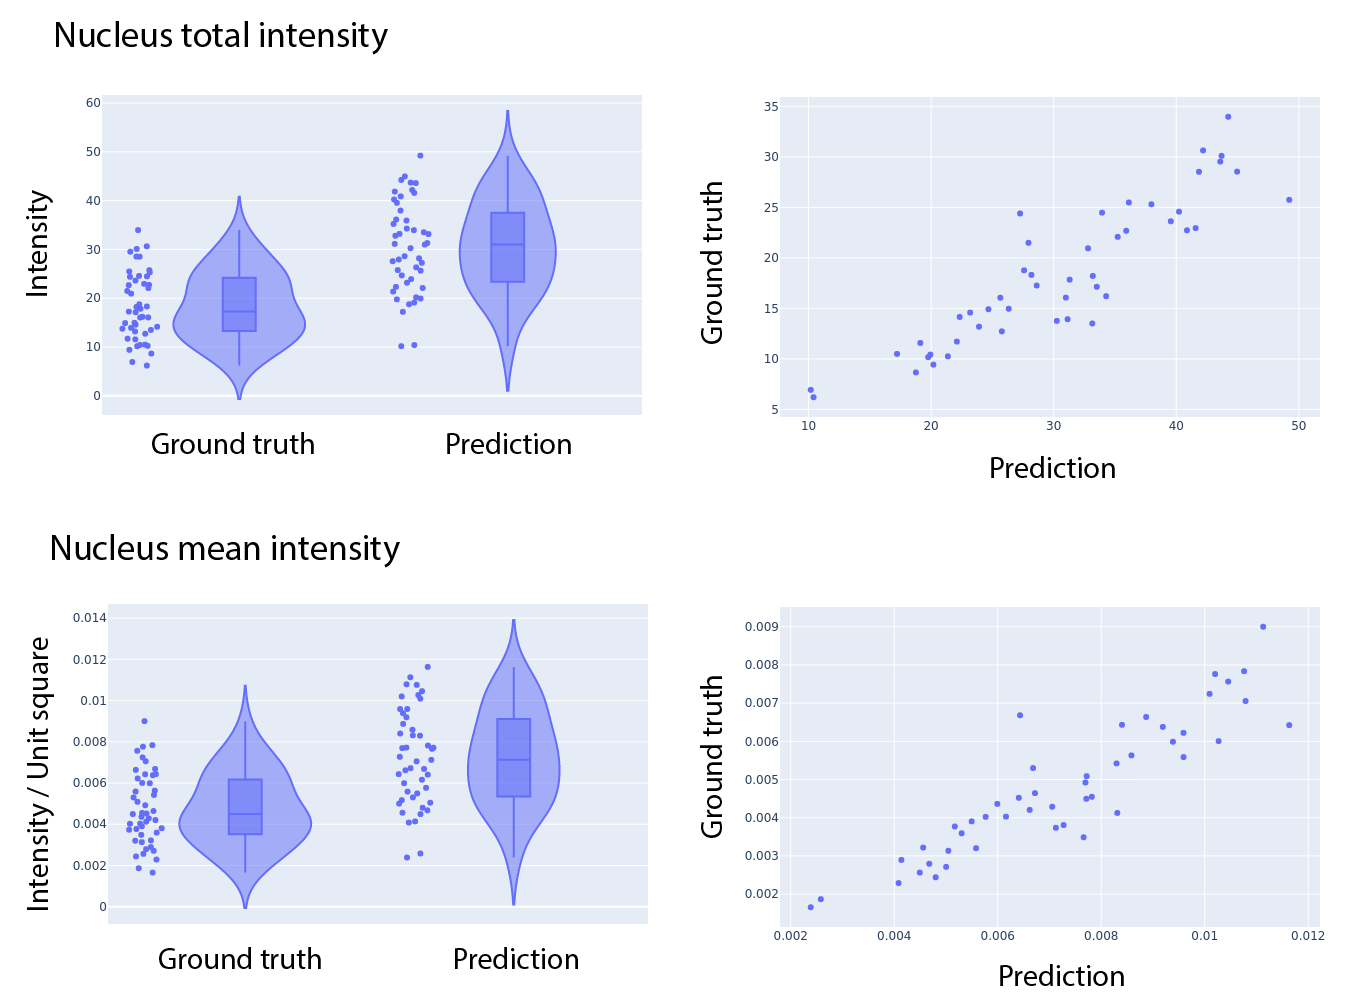
\includegraphics[width=0.8\linewidth]{bilder/nuclei/metric/combined-metrics-2.png}
		\caption{Metrics for practical biological evaluation on nuclei. Total and mean intensities}\label{fig:nuclei-downstream-metrics-1}
	\end{center}
\end{figure}

In general, based on these plots it was concluded that predictions are strongly correlated with the ground truth images in terms of practical biological metrics. Distributions of number of nuclei and their area are very similar in shape, the corresponding scatter plots form almost linear dependance. Distributions of intensities are less similar, the higher intensity of predicted images is proved here. However, high scores in Pearson and Spearman correlation coefficients (see Table \ref{table:nuclei-downstream-metrics-coefficients}) suggest that there is a strong link between predicted and ground truth intensity. The difference between predictions and ground truth might be caused by an absolute value shift, that can be easily adjusted for.

\begin{figure}[htb]
	\begin{center}
		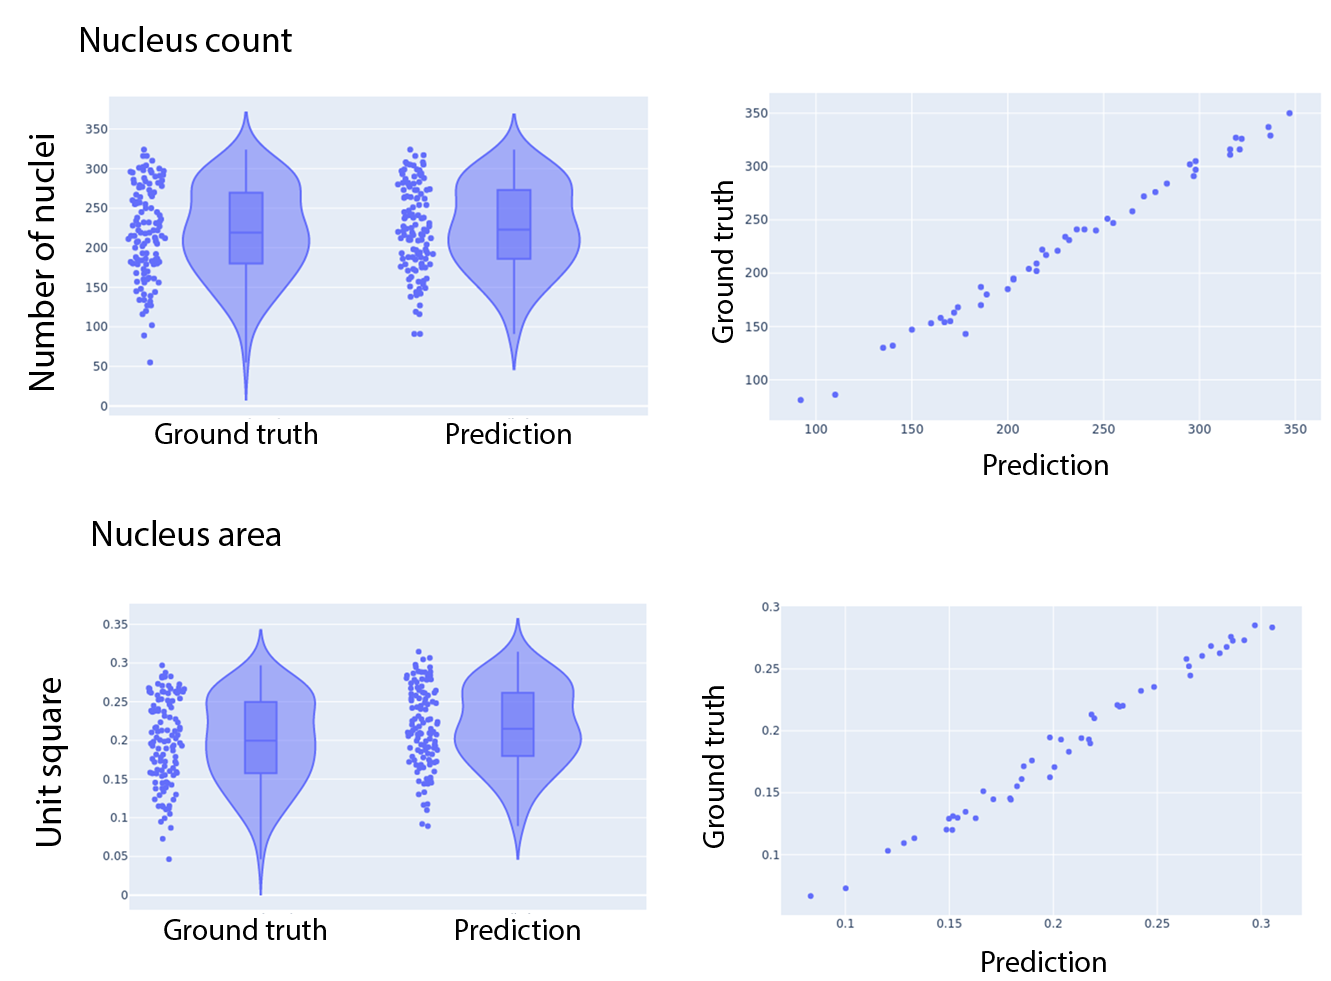
\includegraphics[width=0.8\linewidth]{bilder/nuclei/metric/combined-metrics-1.png}
		\caption{Metrics for practical biological evaluation on nuclei. Count and area}\label{fig:nuclei-downstream-metrics-2}
	\end{center}
\end{figure}

\begin{table}[htb]
    \centering
    \caption{Correlation coefficients for practical biological evaluation on nuclei}
        \begin{adjustbox}{width=0.4\textwidth}
            \begin{tabular}{|c|c|c|}\hline
                &Pearson&Spearman
                \\\hline\hline
                Number of nuclei&0.982&0.984\\\hline
                Total intensity&0.867&0.859\\\hline
                Mean intensity&0.882&0.874\\\hline
                Area&0.971&0.976\\\hline
            \end{tabular}
        \label{table:nuclei-downstream-metrics-coefficients}
        \end{adjustbox}
\end{table}
